\section*{Statistiek deel 2:}

\subsection*{Betrouwbaarheidsintervallen voor het gemiddelde $\mu$ ($\sigma$ bekend)}
    \begin{itemize}
        \item \textbf{\boldmath$100\cdot(1-\alpha)\%$-betrouwbaarheidsinterval (BI) voor \boldmath$\mu$:}
        \[
            z_{\alpha/2} = \text{InvNorm}(\text{opp}=1-\alpha/2; \mu=0; \sigma=1)
        \]
        \[
            [\overline{x} - z_{\alpha/2} \cdot \frac{\sigma}{\sqrt{n}}; \overline{x} + z_{\alpha/2} \cdot \frac{\sigma}{\sqrt{n}}]
        \]

        \item \textbf{Minimale steekproefomvang voor \boldmath$100\cdot(1-\alpha)\%$-BI als \boldmath$\mu$ maximaal \boldmath$\pm a$ mag afwijken:}
        \[
            n \ge \left( \frac{z_{\alpha/2} \cdot \sigma}{a} \right)^2
        \]
    \end{itemize}

\subsection*{Betrouwbaarheidsintervallen voor het gemiddelde $\mu$ ($\sigma$ onbekend)}
    \begin{itemize}
        \item \textbf{\boldmath$100\cdot(1-\alpha)\%$-betrouwbaarheidsinterval (BI) voor \boldmath$\mu$:}
            \[
                t = \invt(\text{opp}=1-\alpha/2; \text{df}=n-1)
            \]
            \[
                [\overline{x} - t \cdot \frac{s}{\sqrt{n}}; \overline{x} + t \cdot \frac{s}{\sqrt{n}}]
            \]

        \item \textbf{Minimale steekproefomvang voor $100\cdot(1-\alpha)\%$-BI als $\mu$ maximaal \boldmath$\pm a$ mag afwijken:}
            \[
                \text{GR tabel (voor verschillende $n$):} \quad \frac{s}{\sqrt{n}} \cdot \text{InvT}(\text{opp}=1-\alpha/2; \text{df}=n-1) \le a
            \]
            
            {\itshape NB: zodra $n \ge 30$, vallen de normale en de $t$-verdeling nagenoeg samen. Je mag dan rekenen met de schatting $s$ in plaats van de daadwerkelijke (onbekende) $\sigma$.}
    

    \item {\bfseries Onderscheidend vermogen (toets met $H_0: \mu=\mu_0$ vs. $H_1: \mu \neq \mu_0$, en gegeven $\mu = \mu_1$)}
        \begin{align*}
            1 - \beta = P(\overline{X} \text{ neemt waarde aan in het kritieke gebied} \mid \mu = \mu_1)
        \end{align*}
    \end{itemize}
\subsection*{Betrouwbaarheidsintervallen voor de binomiale succeskans $p$}
    \textbf{Betrouwbaarheidsinterval voor \boldmath$p$ (Clopper-Pearson):}
    Gegeven een binomiale verdeling met $n$ Bernoulli-experimenten en onbekende $p$, en uitkomst $k$.
    \begin{enumerate}
        \item Bereken de succeskans $p_1$ zodat geldt $P(X \le k) = \binomcdf(n; p; k) = \alpha/2$
        \item Bereken de succeskans $p_2$ zodat geldt $P(X \ge k) = 1 - \binomcdf(n; p; k-1) = \alpha/2$
        \item De berekende waarden voor $p_1$ en $p_2$ zijn de grenzen van het Clopper-Pearson interval.
    \end{enumerate}

\subsection*{Hypothesetoetsen}
    \textbf{Stappenplan hypothesetoetsen}
    \begin{enumerate}
        \item Definieer de nulhypothese $H_0$ en de alternatieve hypothese $H_1$.
        \item Bepaal het significantieniveau $\alpha$ (kans op verwerpen van $H_0$ terwijl $H_0$ waar is $\rightarrow$ type-I fout)
        \item Verzamel data voor de toetsingsgrootheid
        \item Bereken de toetsingsgrootheid
        \begin{itemize}
            \item Uitgaande van de nulhypothese $H_0$ maken we aannames over de kansverdeling van de toetsingsgrootheid!
        \end{itemize}
        \item Geef een conclusie (met behulp van het kritieke gebied / $p$-waarde) en vertaal deze terug naar de originele probleemcontext.
    \end{enumerate}

    \newpage
    \textbf{Drie typen hypothesetoetsen: linkszijdig, tweezijdig, rechtszijdig}
    
    \begin{minipage}{0.32\linewidth}
        \begin{center}
            {\bfseries Linkszijdige toets}
            
            Kritiek gebied:
            
            {\color{red} $(-\infty; g]$}
            
            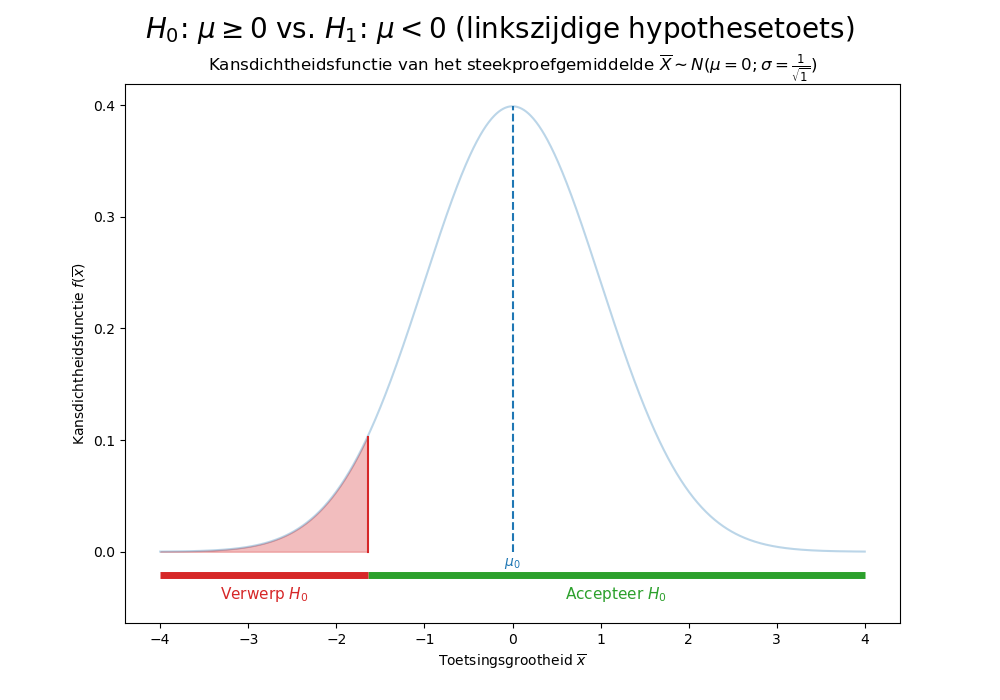
\includegraphics[width=\linewidth]{left_sided.png}
        \end{center}
    \end{minipage}
    \hfill
    \begin{minipage}{0.32\linewidth}
        \begin{center}
            {\bfseries Tweezijdige toets}
            
            Kritiek gebied: 
            
            {\color{red} $(-\infty; g_1]$ en $[g_2; \infty)$}
            
            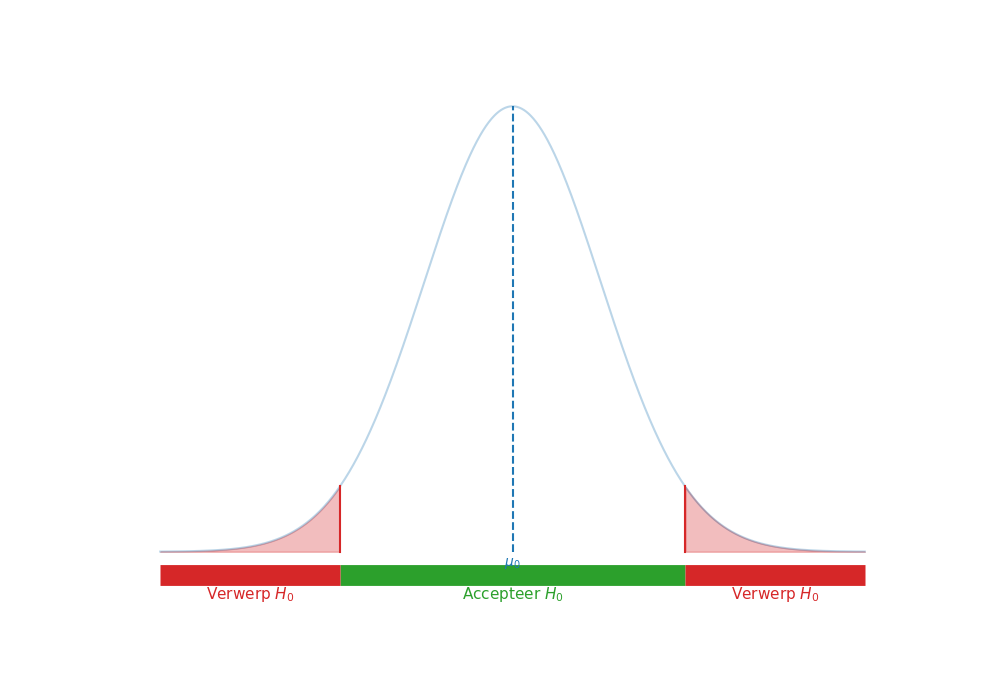
\includegraphics[width=\linewidth]{two_sided.png}
        \end{center}
    \end{minipage}
    \hfill
    \begin{minipage}{0.32\linewidth}
        \begin{center}
            {\bfseries Rechtszijdige toets}
            
            Kritiek gebied:  
            
            {\color{red} $[g; \infty)$}
            
            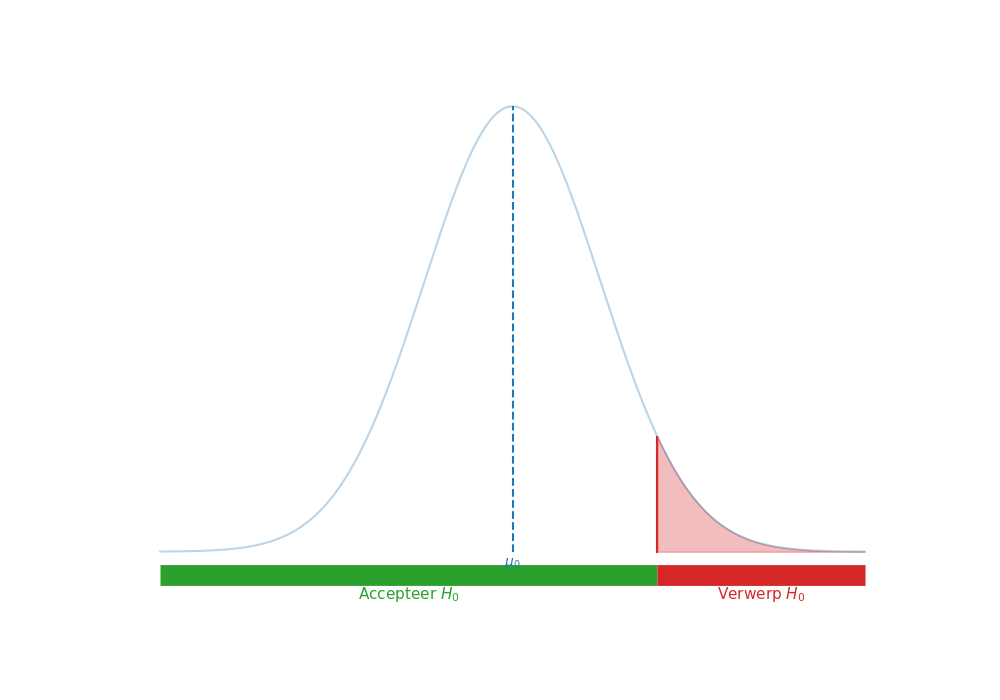
\includegraphics[width=\linewidth]{right_sided.png}
        \end{center}
    \end{minipage}

    \begin{table}[H]
        \centering
        \renewcommand{\arraystretch}{1.5}
        \begin{tabular}{m{2.5cm}|ccc}
            \toprule
                \textbf{Kansverdeling (onder $H_0$)} & \textbf{Linkszijdig} & \textbf{Tweezijdig} & \textbf{Rechtszijdig} \\

            \midrule
                \multirow{2}*{$N(\mu; \sigma)$} & \multirow{2}*{$g = \invnorm(\alpha; \mu; \sigma)$} & $g_1 = \invnorm(\text{opp}=\frac{\alpha}{2}; \mu; \sigma)$ & \multirow{2}*{$g = \invnorm(1-\alpha; \mu; \sigma)$}\\
                & & $g_2 = \invnorm(\text{opp}=1-\frac{\alpha}{2}; \mu; \sigma)$ & \\
            \midrule
                \multirow{2}*{$t(\text{df})$} & \multirow{2}*{$g = \invt(\alpha; \text{df})$} & $g_1 = \invt(\text{opp}=\frac{\alpha}{2}; \text{df})$ & \multirow{2}*{$g = \invt(1-\alpha; \text{df})$}\\
                & & $g_2 = \invt(\text{opp}=1-\frac{\alpha}{2}; \text{df})$ & \\
            \midrule
                \multicolumn{4}{c}{\emph{Grenzen die met de solver functie moeten worden opgelost:}} \\
            \midrule
                $\chi^2(\text{df})$ & \multirow{2}*{$\chi^2\text{cdf}(0; g; \text{df}) = \alpha$} & $\chi^2\text{cdf}(0; g_1; \text{df}) = \frac{\alpha}{2}$ & \multirow{2}*{$\chi^2\text{cdf}(g; 10^{99}; \text{df}) = \alpha$}\\
                (chikwadraat) & & $\chi^2\text{cdf}(g_2; 10^{99}; \text{df}) = \frac{\alpha}{2}$ & \\
            \midrule
                $F(\text{df}_A; \text{df}_B)$ & \multirow{2}*{$\text{Fcdf}(0; g; \text{df}_A; \text{df}_B) = \alpha$} & $\text{Fcdf}(0; g_1; \text{df}_A; \text{df}_B) = \frac{\alpha}{2}$ & \multirow{2}*{$\text{Fcdf}(g; 10^{99}; \text{df}_A; \text{df}_B) = \alpha$}\\
                & & $\text{Fcdf}(g_2; 10^{99}; \text{df}_A; \text{df}_B) = \frac{\alpha}{2}$ & \\
            \bottomrule
        \end{tabular}
    \end{table}

    \textbf{$p$-waardes uitrekenen (gegeven een theoretische en geobserveerde toetsingsgrootheid $T$ en $t$)}
    \begin{table}[H]
        \centering
        \renewcommand{\arraystretch}{1.5}
        \begin{tabular}{m{2.5cm}|cc}
            \toprule
                \textbf{Kansverdeling (onder $H_0$)} & \textbf{Linkszijdig ($P(T \le t)$)} & \textbf{Rechtszijdig ($P(T \ge t)$)} \\
            \midrule
                $N(\mu; \sigma)$ & $p = \normalcdf(-10^{99}; t; \mu; \sigma)$ & $p = \normalcdf(t; 10^{99}; \mu; \sigma)$ \\
            \midrule
                $t(\text{df})$ & $p = \tcdf(-10^{99}; t; \text{df})$ & $p = \tcdf(t; 10^{99}; \text{df})$\\
            \midrule
                $\chi^2(\text{df})$ & $p = \chi^2\text{cdf}(0; t; \text{df})$ & $p = \chi^2\text{cdf}(t; 10^{99}; \text{df})$ \\
            \midrule
                $F(\text{df}_A; \text{df}_B)$ & $p = \text{Fcdf}(0; t; \text{df}_A; \text{df}_B)$ & $p = \text{Fcdf}(t; 10^{99}; \text{df}_A; \text{df}_B)$ \\
            \bottomrule
        \end{tabular}
    \end{table}

    {\itshape NB: Om met de $p$-waarde een conclusie te trekken uit een hypothesetoets vergelijken we de $p$-waarde met het significantieniveau $\alpha$. Let op: bij tweezijdige toetsen neem je het minimum van de linkszijdige en rechtszijdige $p$-waarde en vergelijk je deze met $\alpha/2$!}
    \newpage
    \textbf{Soorten toetsen}
    \begin{table}[H]
        \centering
        \renewcommand{\arraystretch}{1.5}
        \begin{tabular}{c|c|c}
            \toprule
                \textbf{Soort toets} & \textbf{Toetsingsgrootheid} & \textbf{Kansverdeling (onder $H_0$)} \\
            \midrule
                \multicolumn{3}{c}{\textbf{Toetsen voor het gemiddelde $\mu \leq \mu_0$ of $\mu = \mu_0$ of $\mu \geq \mu_0$}} \\ 
            \midrule
                $z$-toets ($\sigma$ bekend)    & $\overline{X}$ & $N(\mu_0; \frac{\sigma}{\sqrt{n}})$ \\
                $t$-toets ($\sigma$ onbekend)  & $T = \frac{\overline{X} - \mu_0}{\frac{s}{\sqrt{n}}}$ & $t(\text{df}=n-1)$ \\
            \midrule
                \multicolumn{3}{c}{\textbf{Chikwadraattoetsen ($\chi^2$)}} \\
            \midrule
                Onafhankelijkheid & $X^2 = \sum_{i,j} \frac{(O_{ij} - E_{ij})^2}{E_{ij}}$ & $\chi^2(\text{df}=\text{(\#rijen-1)} \cdot \text{(\#kolommen-1)})$ \\
                Aanpassing (goodness-of-fit) & $X^2 = \sum_{i} \frac{(O_{i} - E_{i})^2}{E_{i}}$ & $\chi^2(\text{df}=\text{(\#categorie\"en-1)})$ \\
            \midrule
                \multicolumn{3}{c}{\textbf{Verschiltoetsen (op basis van twee populaties $A$ en $B$)}} \\
            \midrule
                $F$-toets: $\sigma_A^2 = \sigma_B^2$ & $F = \frac{S_A^2}{S_B^2}$ & $F(\text{df}_A, \text{df}_B)$ \\
                $z$-toets & $V =\overline{X_A} - \overline{X_B}$ & $N\left(\mu_A - \mu_B; \sqrt{\frac{\sigma_A^2}{n} + \frac{\sigma_B^2}{m}}\right)$ \\
                $t$-toets ($\sigma_A^2 = \sigma_B^2$) & $T = \frac{(\overline{X_A} - \overline{X_B}) - (\mu_A - \mu_B)}{\sqrt{\frac{S_P^2}{n} + \frac{S_P^2}{m}}}$ & $t(\text{df}=n+m-2)$ \\
                $t$-toets ($\sigma_A^2 \neq \sigma_B^2$) & $T = \frac{(\overline{X_A} - \overline{X_B}) - (\mu_A - \mu_B)}{\sqrt{\frac{S_A^2}{n} + \frac{S_B^2}{m}}}$ & $t(\text{df}=\min(n-1;m-1))$ \\
            \bottomrule
        \end{tabular}
    \end{table}

    \textbf{Beslisboom verschiltoetsen}

    \begin{tikzpicture}[node distance=4cm]

        % Nodes
        \node (sigmaKnown) [process] {$\sigma_A$ en $\sigma_B$ bekend?};
        \node (ztest) [process, below of=sigmaKnown, xshift=-4cm, align=center] {Voer $z$-toets uit met \\[1ex] $\displaystyle V = \overline{X_A} - \overline{X_B} \sim N\left(\mu_A - \mu_B; \sqrt{\frac{\sigma_A^2}{n} + \frac{\sigma_B^2}{m}}\right)$};
        \node (varEqual) [process, below of=sigmaKnown, xshift=4cm, align=center] {Voer $F$-toets uit \\[1ex] Wordt $H_0: \sigma_A^2 = \sigma_B^2$ geaccepteerd?};
        \node (pooledT) [process, below of=varEqual, xshift=-4cm, yshift=-1.5cm, align=center] {Voer $t$-toets ($\sigma_A^2 = \sigma_B^2$) uit \\ met ``pooled variance'' \\[1ex] $\displaystyle s_P^2 = \frac{(n-1)\cdot s_A^2 + (m-1) \cdot s_B^2}{n-1+m-1}$ \\[1ex] $\displaystyle t = \frac{(\overline{x_A}-\overline{x_B})-(\mu_A-\mu_B)}{\sqrt{\frac{s_P^2}{n} + \frac{s_P^2}{m}}}$ \\[1ex] $\text{df} = n+m-2$};
        \node (welchT) [process, below of=varEqual, xshift=2cm, yshift=-1.5cm, align=center] {Voer $t$-toets ($\sigma_A^2 \neq \sigma_B^2$) uit \\[1ex] $\displaystyle t = \frac{(\overline{x_A} - \overline{x_B}) - (\mu_A - \mu_B)}{\sqrt{\frac{s_A^2}{n} + \frac{s_B^2}{m}}}$ \\[1ex] $\text{df} = \min(n-1, m-1)$}; % \\ ($\text{df}=\min(n-1; m-1)$)};

        % Arrows
        \draw [arrow] (sigmaKnown) -- node[above, sloped] {ja} (ztest);
        \draw [arrow] (sigmaKnown) -- node[above, sloped] {nee} (varEqual);
        \draw [arrow] (varEqual) -- node[above, sloped] {ja} (pooledT);
        \draw [arrow] (varEqual) -- node[above,sloped] {nee} (welchT);

    \end{tikzpicture}

\newpage

\subsection*{Correlatie en regressie}

\textbf{Correlatieco\"effici\"ent van Pearson:}
\[
    r = \frac{\overline{xy} - \overline{x} \cdot \overline{y}}{\sqrt{(\overline{x^2} - \overline{x}^2)\cdot(\overline{y^2} - \overline{y}^2)}}
\]

\textbf{Correlatieco\"effici\"ent van Spearman:}
\[
    r_s = 1 - \frac{6 \cdot \sum_i d_i^2}{n^3-n}
\]

\textbf{Co\"effici\"enten van de lineaire regressielijn $Y = a + b\cdot X$:}
\begin{align*}
    b &= \frac{\overline{xy} - \overline{x} \cdot \overline{y}}{\overline{x^2} - (\overline{x})^2} \\
    a &= \overline{y} - b \cdot \overline{x}
\end{align*}

\textbf{Schatting van de variantie van de storingsterm $\varepsilon$:}
\begin{align*}
    s_{\varepsilon}^2 &= \frac{\sum e_i^2}{n - 2} = \frac{\sum \left(y_i - (a + b \cdot x_i)\right)^2}{n - 2}=  \frac{n}{n-2} \cdot \left( \overline{y^2} - a \cdot \overline{y} - b \cdot \overline{xy} \right) \\ 
\end{align*}

\textbf{\boldmath$100\cdot(1-\alpha)\%$-betrouwbaarheidsinterval voor de gemiddelde $Y$ bij een gegeven $X = x_0$:}
\[
    t = \invt(\text{opp} = 1 - \alpha/2; \text{df} = n - 2)
\]
\[
    s_\mu = s_{\varepsilon} \cdot \sqrt{ \frac{1}{n} \cdot \left( 1 + \frac{(x_0 - \overline{x})^2}{\overline{x^2} - \overline{x}^2} \right) }
\]
\[
    [a+b\cdot x_0 - t \cdot s_\mu; a+b\cdot x_0 + t \cdot s_\mu]
\]

\textbf{\boldmath$100\cdot(1-\alpha)\%$-betrouwbaarheidsinterval voor $Y$ bij een gegeven $X = x_0$:}
\[
    t = \invt(\text{opp} = 1 - \alpha/2; \text{df} = n - 2)
\]
\[
    s_f = s_{\varepsilon} \cdot \sqrt{ 1 + \frac{1}{n} \cdot \left( 1 + \frac{(x_0 - \overline{x})^2}{\overline{x^2} - \overline{x}^2} \right) }
\]
\[
    [a+b\cdot x_0 - t \cdot s_f; a+b\cdot x_0 + t \cdot s_f]
\]

% \textbf{Covariance:}
% \[
%     Cov(X, Y) = E[(X-E[X])\cdot(Y-E[Y])] = E[X\cdot Y] - E[X]E[Y]
% \]

% \textbf{Correlation coefficient:}
% \[
%     \rho(X, Y) = \frac{Cov(X,Y)}{\sqrt{Var(X) \cdot Var(Y)}}
% \]

% \textbf{Variance of error terms:}
% \[ \hat{\sigma}^2 = \frac{1}{n-2}\sum_{i=1}^{n} (y_{i} - \hat{y}_{i})^2 = \frac{\sum_{i=1}^{n} y_{i}^2 - \hat{\beta}_{0}\cdot \sum_{i=1}^{n} y_{i} - \hat{\beta}_{1}\cdot \sum_{i=1}^{n} x_{i}y_{i}}{n-2}\]

% \textbf{Coefficients of regression line:}

% Given a sample of $n$ observations $(x_1, y_1), (x_2, y_2), \ldots, (x_n, y_n)$, the regression line $\hat{y} = \hat{\beta}_0 + \hat{\beta}_{1}\cdot x$ satisfies:
% \begin{itemize}
%     \item $\hat{\beta}_{1} = \frac{\sum_{i=1}^{n}x_iy_i - n \cdot \overline{x} \cdot \overline{y}}{\sum_{i=1}^{n} x_{i}^2 - n \cdot \overline{x}^2}$
%     \item $\hat{\beta}_{0} = \overline{y} - \hat{\beta}_{1} \cdot \overline{x}$
% \end{itemize}

% \textbf{Sample correlation coefficient:}
% \[ r(X, Y) = \frac{Cov(X, Y)}{\sqrt{s_{X}^2\cdot s_{Y}^2}} = \frac{\sum_{i=1}^{n}(x_{i}-\overline{x})\cdot(y_{i} - \overline{y})}{\sqrt{\sum_{i=1}^{n}(x_{i}-\overline{x})^2 \cdot \sum_{i=1}^{n}(y_{i}-\overline{y})^2}} = \frac{\sum_{i=1}^{n}x_{i}y_{i} - n \cdot \overline{x}\cdot \overline{y}}{\sqrt{\left(\sum_{i=1}^{n}x_{i}^2-n\cdot \overline{x}^2\right) \cdot \left(\sum_{i=1}^{n}y_{i}^2-n\cdot \overline{y}^2\right)}}\]

% \textbf{Likelihood function:}
% \[ L(x_1, x_2, \ldots, x_n; \theta) = f(x_1; \theta)\cdot f(x_2; \theta)\cdot\ldots\cdot f(x_n; \theta)\]

% \textbf{Minimum sample size with given accuracy $E$:}
% \[ n \ge \left(\frac{z_{\frac{\alpha}{2}} \cdot \sigma}{E}\right)^2\]

% \textbf{Minimum sample size for bounding type II error $\beta$}
% \[ n \ge \frac{(z_{\frac{\alpha}{2}}+z_{\beta})^2 \cdot \sigma^2}{\delta^2}\]

% \textbf{Veelgebruikte functies op de grafische rekenmachine}
% \begin{table}[H]
%     \centering
%     \begin{tabular}{c|c|c}
%         \toprule
%             \textbf{Vraag}                     & \textbf{TI-84 Plus}           & \textbf{Casio} \\
%         \midrule
%             \multicolumn{3}{c}{\textbf{Continue kansverdeling (willekeurig)}} \\ 
%         \midrule
%             $z_{p}$                      & invNorm$(\text{opp}=1-p; \mu=0; \sigma=1)$      & InvNormCD$(\text{opp}=1-p; \sigma=1; \mu=0)$\\
%             $t_{p}$                      & invNorm$(\text{opp}=1-p; \mu=0; \sigma=1)$      & InvNormCD$(\text{opp}=1-p; \sigma=1; \mu=0)$\\
%         \midrule    
%             \multicolumn{3}{c}{\textbf{$X \sim \text{Binomiaal}(n, p)$}} \\ 
%         \midrule
%             $P(X = k)$                              & binompdf$(n,p,k)$             & BinomialPD$(k, n, p)$ \\
%             $P(X \le k)$                            & binomcdf$(n,p,k)$             & BinomialCD$(k, n, p)$ \\
%         \midrule    
%             \multicolumn{3}{c}{\textbf{$X \sim N(\mu, \sigma)$}} \\
%         \midrule 
%             $P(a \le X \le b)$                      & normalcdf$(a,b,\mu,\sigma)$   & NormalCD$(a, b, \sigma, \mu)$ \\
%             % Grenswaarde $g$ zodat $P(X \le g)=p$?   & invNorm$(p,\mu,\sigma)$       & InvNormCD$(\text{tail=left}, p, \sigma, \mu)$ \\
%         \midrule 
%             \multicolumn{3}{c}{\textbf{$X \sim \text{Poisson}(\lambda)$}} \\  
%         \midrule
%             $P(X = k)$                              & poissonpdf$(\lambda, k)$      & PoissonPD$(k, \lambda)$ \\
%             $P(X \le k)$                            & poissoncdf$(\lambda, k)$      & PoissonCD$(k, \lambda)$ \\
%         \bottomrule
%     \end{tabular}
% \end{table}

\end{document}
